\section{Background}
\label{sec:overview}

We review the background in stateless model checking and data-race analysis using the example program in Figure~\ref{fig:example}.

\begin{figure}[t]
	\small
\begin{tabular}{rll}
	& \multicolumn{2}{c}{\texttt{int x = 0; mutex\_t mx;}} \\
	& {\bf Thread 1} & {\bf Thread 2} \\
	1 & \texttt{\hilight{orange}{mutex\_lock(\&mx);}} & \\
	2 & \texttt{int tmp = x;} &\\
	3 & & \texttt{atomic\_xadd(\&x, 1);} \\
	4 & & \texttt{\hilight{olivegreen}{yield();}} \\
	5 & & \texttt{atomic\_xadd(\&x, 1);} \\
	6 & \texttt{x = tmp + 1;} & \\
	7 & \texttt{\hilight{commentblue}{mutex\_unlock(\&mx);}} & \\
	8 & \texttt{assert(x >= 1);}  & \\
	9 & & \texttt{assert(x >= 2);} \\
	%1 & \texttt{\hilight{brickred}{x->foo = ...;}} & \\
	%2 & \texttt{\hilight{olivegreen}{free}(x);} \\
	%3 & & \texttt{\hilight{commentblue}{// x's memory recycled}} \\
	%4 & & \texttt{y~=~\hilight{olivegreen}{malloc}(sizeof *y);} \\
	%5 & & \texttt{\hilight{commentblue}{// ...initialize...}}\\
	%6 & & \texttt{publish(y);} \\
	%7 & & \texttt{\hilight{brickred}{y->bar = ...;}} \\
\end{tabular}
\caption{Example program with a data-race bug. In this interleaving, the assertion on line 9 will fail. Two data-race preemptions are required to expose the bug: one just before thread 1's line 6, and one just before thread 2's line 9.}
\label{fig:example}
\end{figure}

\subsection{Stateless Model Checking}

Stateless model checking \cite{verisoft} is a testing technique for systematically exploring the possible thread interleavings of a concurrent program.
A stateless model checker executes the program repeatedly, each time according to a new thread interleaving, until the state space (or the CPU budget) is exhausted.
Rather than identifying suspicious conditions which may include false alarms, the approach of many static analyses \cite{racerx,coverity},
stateless model checkers focus on concrete observable failures such as assertions, deadlocks, and segfaults.

\begin{figure}[t]
	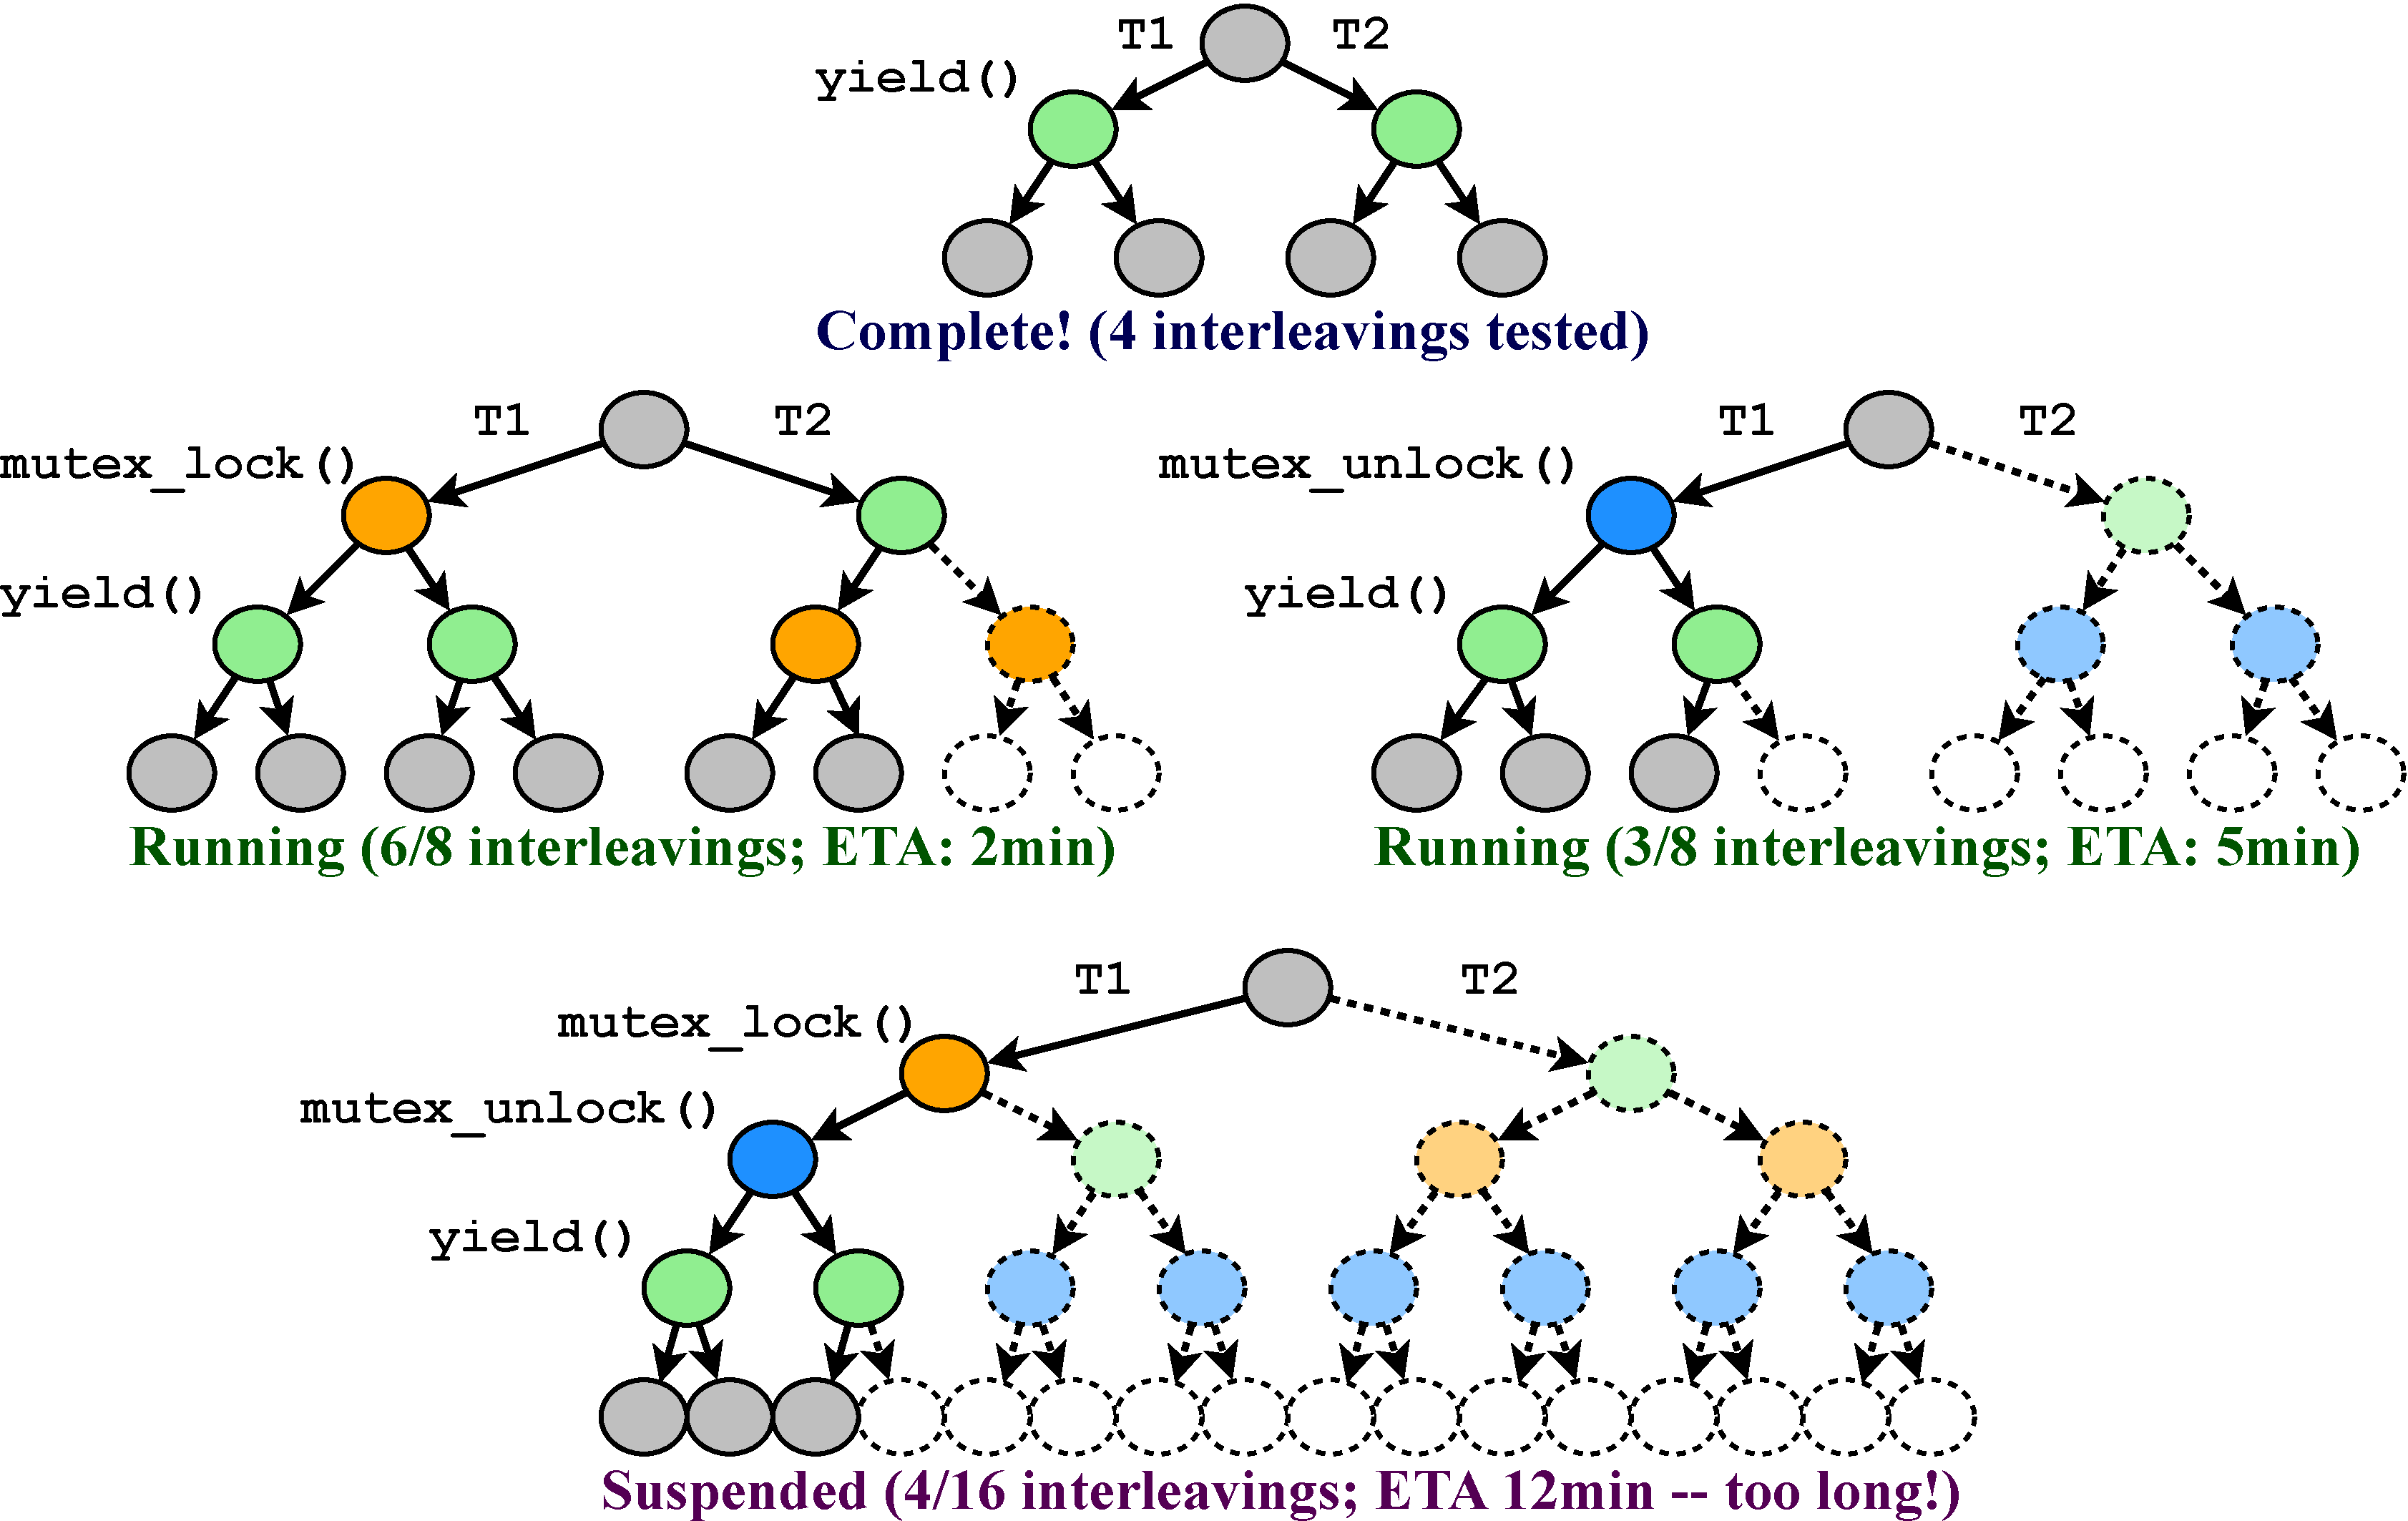
\includegraphics[width=0.48\textwidth]{trees-v2-squashed.pdf}
	\caption{Iterative Deepening example.
		The minimal state space (top) includes only voluntary thread switches, such as {\tt yield()}. %or {\tt cond\_wait()}.
		Multiple further tests can be run: preempting on calls to {\tt mutex\_lock} alone (left), {\tt mutex\_unlock} alone (right), or both together (bottom).
Each option increases the state space size unpredictably, so multiple state spaces should be tested in parallel.
Estimation techniques~\cite{estimation} inform which state spaces to prioritize.
}
	\label{fig:id}
\end{figure}

The checker defins the granularity of thread interleavings by which {\em preemption points} it uses to switch threads.
Most model checkers \cite{chess} choose synchronization/thread library API boundaries for these points;
in our example program, these would be lines 1, 4, and 7.
Figure~\ref{fig:id} shows several possible resulting state spaces.
The approach of prior work is to enable all preemption points simultaneously, i.e., to test only the bottom state space.

To mitigate the exponential explosion,
Dynamic Partial Order Reduction \cite{dpor} identifies equivalent execution sequences according to Mazurkiewicz trace theory \cite{mazurkiewicz},
and tests at least one execution from each equivalence class.
Intuitively, if two thread transitions between preemption points do not conflict on any shared resource access, reordering them produces an equivalent interleaving.
Nevertheless, state spaces are still exponentially-sized in the number of conflicting transitions.

This motivates {\em Iterative Deepening}, our new technique for adjusting the preemption points at runtime.
Rather than committing to one state space with every available preemption point enabled,
Iterative Deepening searches among different {\em subsets} of the points;
for example, ``preempt on all calls to {\tt mutex\_lock} but not on {\tt mutex\_unlock}''.
Hence, we will test all the state spaces shown in Figure~\ref{fig:id} in parallel,
and decide on-the-fly whether to pursue each test, or to defer it in favour of smaller ones.

\subsection{Data Race Detection}

Data race analysis \cite{eraser} identifies pairs of unsynchronized memory accesses between threads.
Two instructions are said to race if
they both access the same memory address,
at least one is a write,
the threads do not hold the same lock,
and no synchronization enforces the order of the thread transitions.
Data races are not necessarily bugs, but represent suspicious violations of the locking discipline.
In Figure~\ref{fig:example}, lines 3 and 5 each race with 2, 6, and 8, and line 6 races with 9.

Though state-of-the-art MCs preempt only on synchronization events,
many serious concurrency bugs are caused by data races leading to corrupted shared state.
Figure~\ref{fig:example}'s thread interleaving is possible only with {\em data-race preemption points}:
preempting a thread just before an instruction identified as part of a data race.
None of the state spaces in Figure~\ref{fig:id} contain this interleaving,
as none of the mutex/yield preemptions split lines 2 and 6 across different transitions.

\subsection{Terminology}

For the rest of the paper, we will abbreviate {\em preemption point} (PP),
%For the remainder of the paper, we will abbreviate {\em preemption point} (PP),
{\em model checking} (MC),
{\em single-state-space model checking} (SSS-MC), % (i.e., the approach of prior work),
Dynamic Partial Order Reduction (DPOR), and {\em state space estimate} (ETA).

SSS-MC indicates the approach of prior model checking tools:
the set of PPs is fixed in advance, and the tool commits to testing every interleaving available with those PPs.
%Reduction techniques are often used to skip equivalent interleavings \cite{dpor}, and search-ordering strategies
Many techniques exist to skip equivalent interleavings and order the search to uncover bugs faster \cite{dpor,demeter,chess-icb,gambit},
but new PPs cannot be added, nor ineffective ones removed, by any dynamic analysis.

We distinguish between data-race {\em candidates} and data-race {\em bugs}.
Because data-race analysis is prone to false-positives,
we classify unprotected access pairs separately from bugs,
calling such pairs {\em data race candidates}.
Should a future interleaving, preempting during those accesses,
lead to a failure, then we report a {\em data-race bug}.
Otherwise, if the access pair can be reordered, but does not produce a failure under any interleaving, it is a {\em benign data race}.
If they cannot be reordered at all, it is a {\em false positive}.
%TODO: Don't do this, below. Scan paper for uses of 'false positive' where you mean to say 'benign' or 'both'.
%For brevity, we count benign data races as a subset of false positives.

We also identify the {\em minimal} and {\em maximal state space} for each test.
The {\em minimal state space} includes only thread switches arising from normal execution (Figure~\ref{fig:id}, top).
The {\em maximal state space} is the one tested by SSS-MC: all statically-available PPs are enabled (Figure~\ref{fig:id}, bottom).
%However, should new data-race PPs be added during a test, the new maximal state space will be the one including those as well.
%% don't say this ^ -- because when you add dr pps, they add in pairs and there would be multiple maximals, at least until they each get explored and subseuqnetly add a pp of the other of the pair.
